\let\negmedspace\undefined
\let\negthickspace\undefined
\documentclass[journal]{IEEEtran}
\usepackage[a5paper, margin=10mm, onecolumn]{geometry}
%\usepackage{lmodern} % Ensure lmodern is loaded for pdflatex
\usepackage{tfrupee} % Include tfrupee package

\setlength{\headheight}{1cm} % Set the height of the header box
\setlength{\headsep}{0mm}     % Set the distance between the header box and the top of the text

\usepackage{gvv-book}
\usepackage{gvv}
\usepackage{cite}
\usepackage{amsmath,amssymb,amsfonts,amsthm}
\usepackage{algorithmic}
\usepackage{graphicx}
\usepackage{textcomp}
\usepackage{xcolor}
\usepackage{txfonts}
\usepackage{listings}
\usepackage{enumitem}
\usepackage{mathtools}
\usepackage{gensymb}
\usepackage{comment}
\usepackage[breaklinks=true]{hyperref}
\usepackage{tkz-euclide} 
\usepackage{listings}
% \usepackage{gvv}                                        
\def\inputGnumericTable{}                                 
\usepackage[latin1]{inputenc}                                
\usepackage{color}                                            
\usepackage{array}                                            
\usepackage{longtable}                                       
\usepackage{calc}                                             
\usepackage{multirow}                                         
\usepackage{hhline}                                           
\usepackage{ifthen}                                           
\usepackage{lscape}
\usepackage{circuitikz}
\tikzstyle{block} = [rectangle, draw, fill=blue!20, 
    text width=4em, text centered, rounded corners, minimum height=3em]
\tikzstyle{sum} = [draw, fill=blue!10, circle, minimum size=1cm, node distance=1.5cm]
\tikzstyle{input} = [coordinate]
\tikzstyle{output} = [coordinate]


\begin{document}

\bibliographystyle{IEEEtran}
\vspace{3cm}

\title{3.3.15}
\author{AI25BTECH110031 \\ Shivam Sawarkar}
 \maketitle
% \newpage
% \bigskip
{\let\newpage\relax\maketitle}

\renewcommand{\thefigure}{\theenumi}
\renewcommand{\thetable}{\theenumi}
\setlength{\intextsep}{10pt} % Space between text and floats


\numberwithin{equation}{enumi}
\numberwithin{figure}{enumi}
\renewcommand{\thetable}{\theenumi}

\textbf{Question(3.3.15)}
Construct a triangle ABC in which $BC = 7 cm$, and median $AD = 5 cm$, $\angle A=60^\circ$.
Write the steps of construction also.

\textbf{Solution:} \\ 
\begin{align}
\vec{B}=\myvec{0\\0},\qquad 
\vec{C}=\myvec{7\\0},\qquad 
\vec{D}=\myvec{3.5\\0}.
\end{align}

Since $AD=5$, point $\vec{A}$ lies on the circle with center $\vec{D}$ and radius 5.  
We parametrize:
\begin{align}
\vec{A}=\vec{D}+5\myvec{\cos\theta\\ \sin\theta}
=\myvec{3.5+5\cos\theta\\[4pt]5\sin\theta}.
\end{align}

Define the vectors
\begin{align}
\vec{c}=\vec{AB}=\vec{B}-\vec{A}
=\myvec{-3.5-5\cos\theta\\ -5\sin\theta},\\ 
\vec{b}=\vec{AC}=\vec{C}-\vec{A}
=\myvec{3.5-5\cos\theta\\ -5\sin\theta}.
\end{align}

\textbf{Angle condition:}  
\begin{align}
\vec{c}^\top \vec{b}=\norm{c}\norm{b}\cos60^\circ
=\dfrac{1}{2}\norm{c}\norm{b}
\end{align}

Compute the dot product:
\begin{align}
\vec{c}^\top \vec{b}
=(-3.5-5\cos\theta)(3.5-5\cos\theta)+(-5\sin\theta)(-5\sin\theta)
=\frac{51}{4}.
\end{align}

Hence
\begin{align}
\norm{b}\norm{c}=\frac{51}{2}.
\end{align}

Now,
\begin{align}
\norm{c}^2=\dfrac{149}{4}+35\cos\theta,\qquad
\norm{b}^2=\dfrac{149}{4}-35\cos\theta.
\end{align}

Therefore,
\begin{align}
(\norm{c}\norm{b})^2
=\brak{\dfrac{149}{4}}^2-(35\cos\theta)^2.
\end{align}

Substituting $\norm{c}\;\norm{b}=\dfrac{51}{2}$,
\begin{align}
\brak{\dfrac{51}{2}}^2=\brak{\dfrac{149}{4}}^2-(35\cos\theta)^2,
\end{align}
\begin{align}
\cos^2\theta=\frac{11797}{19600}.
\end{align}

Thus,
\begin{align}
\cos\theta=\pm\frac{\sqrt{11797}}{140},\qquad
\sin\theta=\pm\frac{\sqrt{7803}}{140}.
\end{align}

Finally, coordinates of $A$ are
\begin{align}
\vec{A}=\myvec{
\dfrac{7}{2}\pm\dfrac{\sqrt{11797}}{28}\\ 
\pm\dfrac{\sqrt{7803}}{28}
}.
\end{align}

\begin{figure}[H]
    \centering
    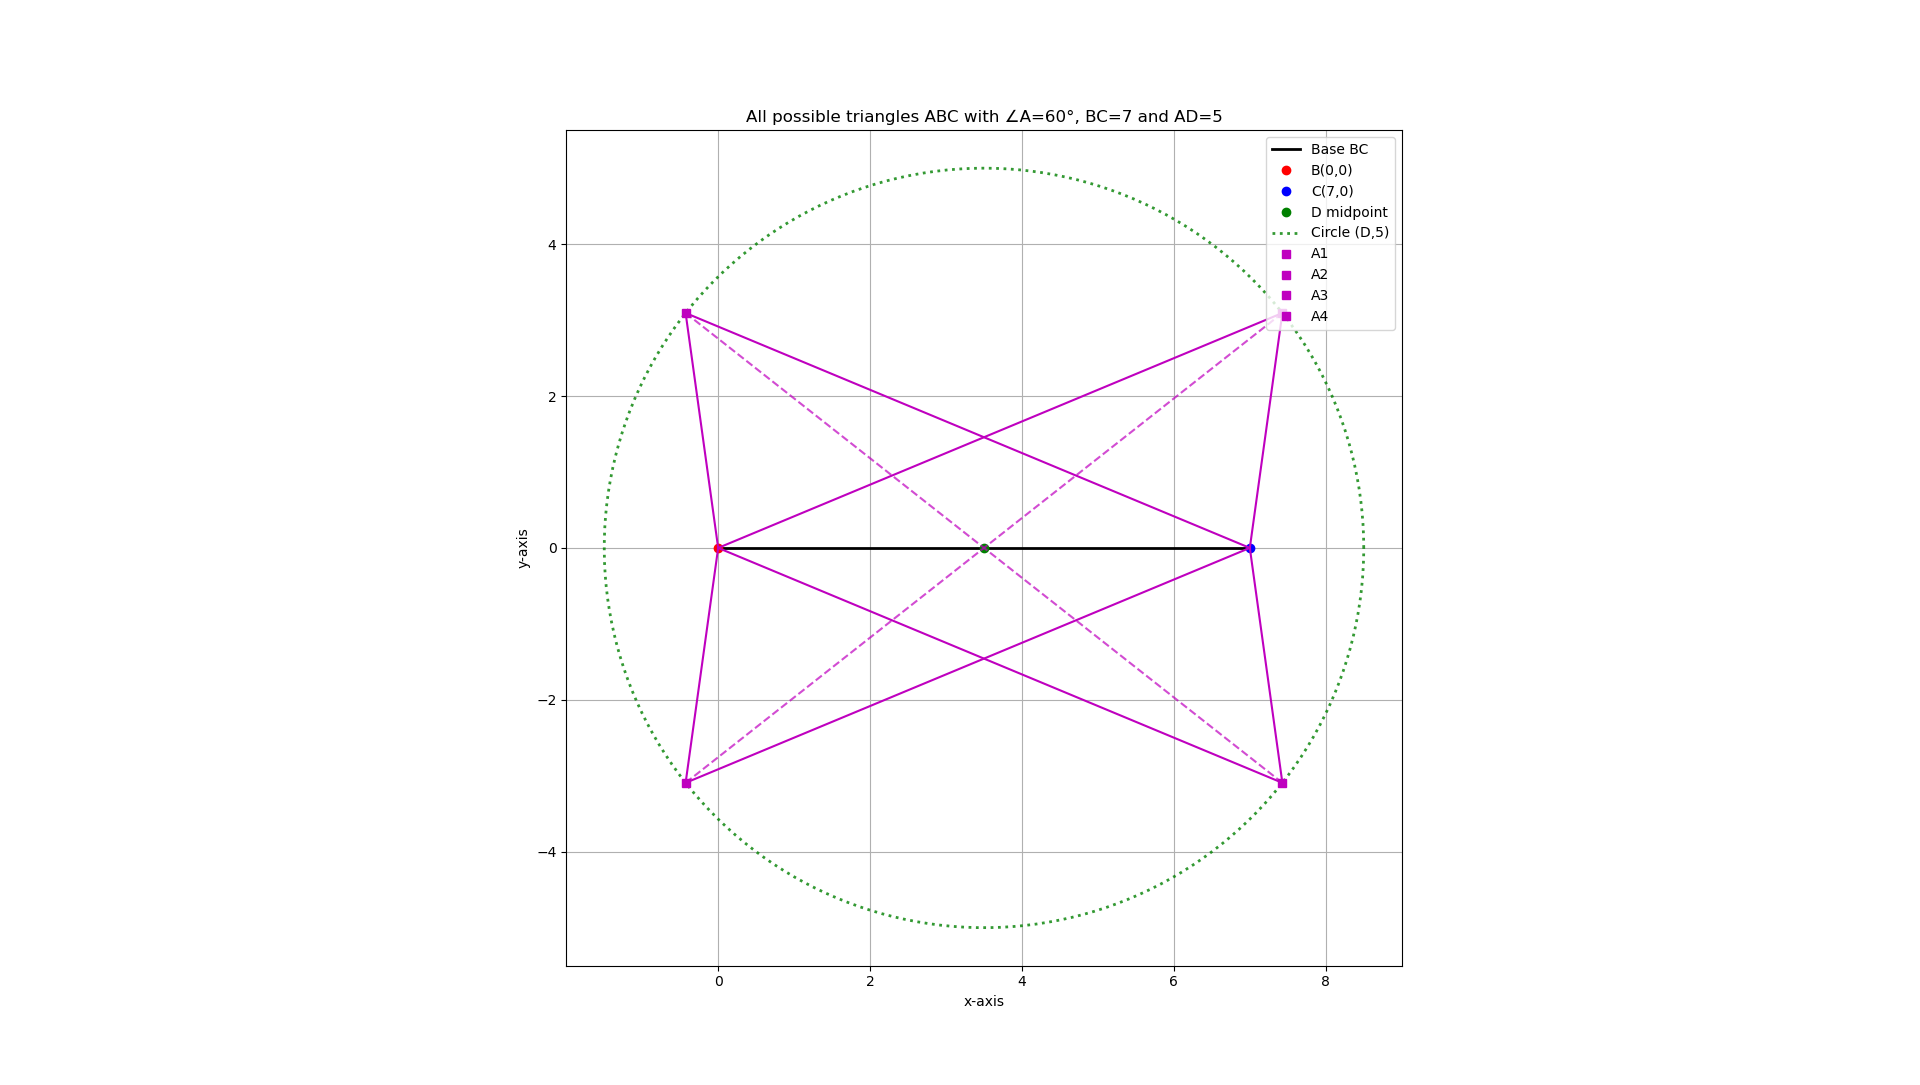
\includegraphics[width=1\linewidth]{figs/plot6.png}
    \caption{}
    \label{fig:placeholder}
\end{figure}





\end{document}